\documentclass{sig-alternate}
%\usepackage{graphicx}

\begin{document}

\title{Geo-Store: A Geospatial-Enabled SPARQL Evaluation Engine}

\numberofauthors{2}
\author{
% 1st. author
\alignauthor
Chih-Jye Wang\\
    \affaddr{Department of CSSE}\\
    \affaddr{Auburn University}\\
    \affaddr{Auburn, AL, USA}\\
    \email{wangchj@auburn.edu}
% 2nd. author
\alignauthor
Wei-Shinn Ku\\
    \affaddr{Department of CSSE}\\
    \affaddr{Auburn University}\\
    \affaddr{Auburn, AL, USA}\\
    \email{weishinn@auburn.edu}
}

\conferenceinfo{GIS'12,} {November 6-9, 2012. Redondo Beach, CA,
USA}\CopyrightYear{2012}

\maketitle

\begin{abstract}
Geo-Store is a geospatial data management system for data expressed in the resource description framework (RDF). Our system implements common spatial query types in terms of SPARQL query filters, which allow user to perform query operations based on spatial relationships. To efficiently evaluating spatial queries, our system implements spatial-aware hashing for geographic data. Geospatial data management in semantic web data is an emerging research field, and our system shows the advantages of integrating GIS with semantic web. For more information, our system can be accessed at http://ilab.auburn.edu/geostore.
\end{abstract}

% A category with the (minimum) three required fields
\category{H.4}{Information Systems Applications}{Miscellaneous}
%A category including the fourth, optional field follows...
\category{D.2.8}{Software Engineering}{Metrics}[complexity measures, performance measures]

\terms{Theory}

\keywords{ACM proceedings, \LaTeX, text tagging} % NOT required for Proceedings

\section{Introduction}

%One of the values of the Hypertext Transfer Protocol (HTTP) often known as the World
%Wide Web is that one document is linked to other documents and relevant information
%can be obtained through the links. Similarly, the semantic web is a relatively new
%field of research and a fledgling set of standards that attempts to create a web of
%linked data in standardized format to help machine readability and processing. The
%web and the semantic web are tightly woven due to that much of semantic data are
%existing data on the web migrated to the new format or obtained by annotating
%the existing web with semantic information .
%
%Much of the semantic web data describe geospatial information, such as location of
%places, and geospatial information system that access this information is able to
%perform
%
%---

Semantic web is a fledgling field of research and set of standards to create a web of machine readable and processable data. The strength of this linked data is that, like the existing web, each piece of information can be linked to other pieces of information each identified by a unique identifier. For example, John could publish his information in the Friend Of A Friend\footnote{http://www.foaf-project.org/} (FOAF) format that is easily readable by machines. John's information may contain his basic information such as name and birthday; in addition, his information may also contain links to his friends in FOAF format, as well as things he like, such as a movie, which could also be uniquely identified and precisely described in semantic format\cite{lee:semantic_web}. In this example, a semantic aware application that has the identifier of John could retrieve information such as ``find all the movies liked by friends of John."

Due to recent research effort and growth, much of the semantic data describe geospatial entities, such as location and geographic extend of objects. Geospatial information systems that access semantic data can make powerful inference based on spatial and non-spatial information from various source and not limited to data of only certain domains. For example, to find a location for a new fast food restaurant, a location planning software needs to find name and location of near by restaurants as well as other types of point of interest, such as schools and shopping malls, within 5 kilometers of radius of candidate locations. The application pulls information from various sources and determines the optimal location. Despite the growth of semantic web data, it is an ongoing research to best manage and query geospatial semantic data to support upcoming applications.

Resource Description Framework (RDF) is a framework for describing entities (also known as \emph{resources} in semantic jargon) in semantic web format. Each property of an entity is described as a triple (S, P, O) consisting a subject, which denotes the entity, a predicate, denoting a property of the entity, and an object, the value of the property. Object of a triple can be either a literal or the subject of another triple (or the identifier of an entity) creating a link between the entities. The linking between entities forms a graph. A system that manages and control access to a set of triple is often called a \emph{triple store}.

The purpose of this paper is to demonstrate Geo-Store~\cite{journals/internet/KuCWL}, a geospatial-enabled triple store. The system implements spatial query filters, which allow user to integrate spatial relationships into SPARQL queries. The system utilizes spatial-aware hashing to efficiently implement these spatial features. In addition, the system provides a query builder for the user to easily compose geospatial queries. Our system utilizes spatial aware indexing to facilitate efficient evaluation of spatial filters. The system is built on top of RDF-3X~\cite{DBLP:journals/vldb/NeumannW10}, a scalable RDF management system. 
%\input{related_works}
\section{System Architecture and Design}

Figure~\ref{fig:architect} shows an overview design of our system. The components of the system is discussed in this section.

\begin{figure}
\centering
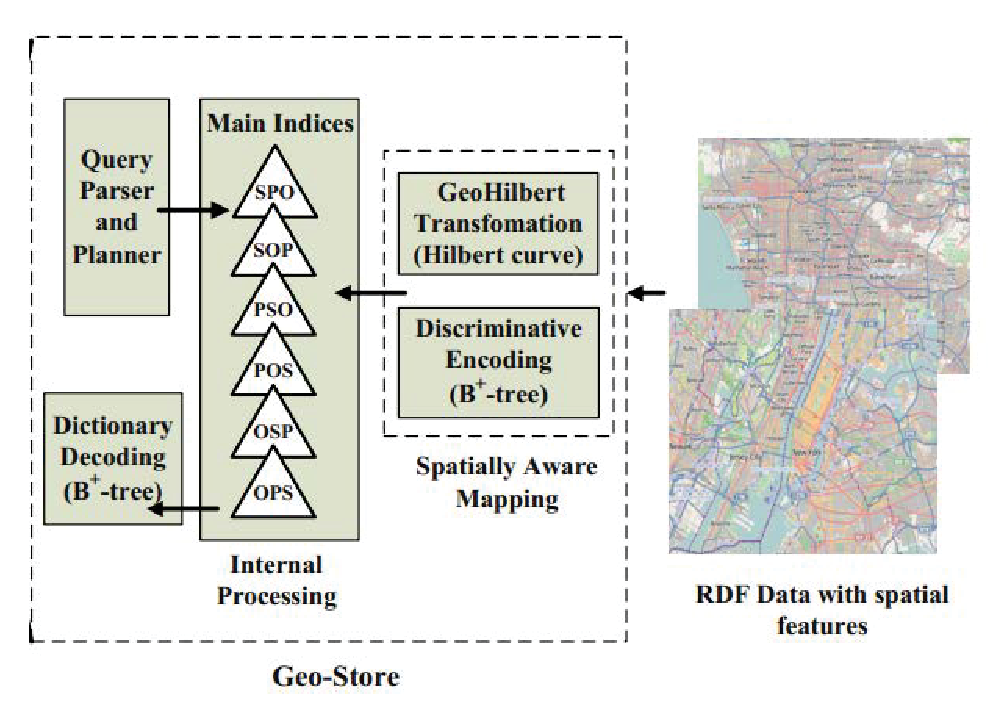
\includegraphics[width=3in]{images/architect.eps}
\caption{Geo-Store System Architecture}\label{fig:architect}
\end{figure}

\subsection{Spatial-Aware Hashing}

In order to support efficient geospatial query processing, the system performs spatial-aware hasshing (SAH) when geo-coordinates is encountered during insertion and update of data. The spatial-aware hasing is based on Hilbert space filling curve transformation, in which a two-dimensional coordinates of a point is transformed into an integer. A benefit of this transformation is to reduce a RDF geo-coodinates literal into a short integer; therefore, eliminating long string comparison during query evaluation. Another benefit is that the transformation produces locality-preserving results, so two points that are ``close" in the original space will have high chance of being hashed to close values. The query evaluator uses this locality-preserving property to approximate spatial extend of spatial constraints of a query.

The result of the a SAH is placed into the underlying data store as a triple, where the subject is the entity of which the location was hashed. The hashed value is then further indexed by B-Tree indexes (shown as Main Indices in Figure~\ref{fig:architect}) for fast look-up.

\subsection{Spatial Query Analyzer}

After the SAH has been performed on newly inserted data, the system can start evaluating queries. When a query is received, the query analyzer looks for spatial filters within the query. When a filter is found, the analyzer uses the same spatial-aware hashing algorithm, described previously, to find a list of spatial hash values (integers) covered by the filter. Since the underlying data store does not aware any spatial context and only understand standard SPARQL patterns, the query analyzer translates the list of hash values into query patterns and removes the translated spatial filter. All these steps essentially adds SPARQL graph patterns to approximate the entities that are covered by the query filter. For multiple query filters within a query, the process is the same for each, but the analyzer performs union for overlapping hash values.

\section{Spatial Queries}

\underline{\textbf{Window Filter}} \\
Window filter constraints the binding of a query variable to within a rectangular region defined by two corners. The follow query is an example.

\begin{verbatim}
SELECT ?name ?location
WHERE{
    ?e <name> ?name.
    ?e <coordinates> ?location.
    within(?location, 32.5955, -85.4909, 32.6122,
           -85.4739)
}
\end{verbatim}
%\caption{\small Skyline SQL Clause.
%\label{fig:skyline_sql}}

\underline{\textbf{Range Filter}} \\
Range filter constraints the binding of a query variable to a circular region a distance from a center.

\begin{verbatim}
SELECT ?name ?location
WHERE{
    ?e <name> ?name.
    ?e <coordinates> ?location.
    within(?location, 32.597178, -85.463086, 1500)
}
\end{verbatim}

\underline{\textbf{Nearby Filter}} \\
Range filter constraints the binding of a query variable to a circular region a distance from a center.

\begin{verbatim}
SELECT ?name ?location
WHERE{
    ?e <name> ?name. ?e <coordinates> ?location.
    nearby(?location, 32.607985, -85.481439, 3)
}
\end{verbatim}

\section{Query Builder}

Figure~\ref{fig:geostore_web} shows the query builder of the system. The interface consists of two parts. The top part is the query editor that allows the user to manually enter the query. Below the editor is the builder tool that assist the user to construct query graph patterns as well as geospatil query filters.

\begin{figure}[t]
\centering
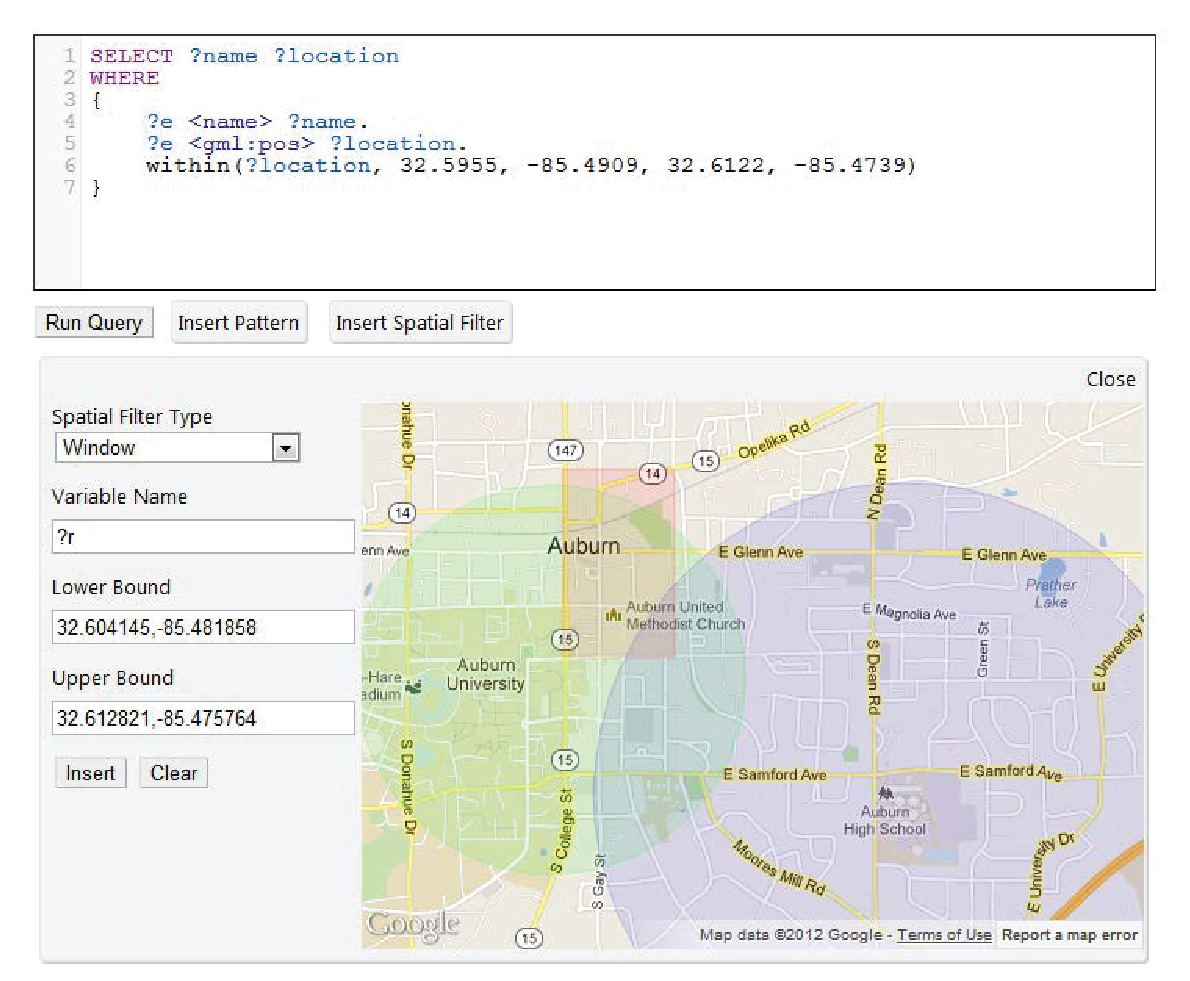
\includegraphics[width=3.3in]{images/geostore_web.eps}
\caption{Geo-Store Query Builder Interface}\label{fig:geostore_web}
\end{figure} 
\section{Conclusions}
In this demonstration, we present Geo-Store, a spatially-aware data management system built on the RDF-3X~\cite{DBLP:journals/vldb/NeumannW10}. By the augmentation of the standard SPARQL language with spatial filters, Geo-Store is able to process complex queries with common spatial constraints. Due to the use of the spatially-aware hashing, Geo-Store manages to provide an efficient solution to evaluate SPARQL queries with spatial constraints without any price on accuracy.

%ACKNOWLEDGMENTS are optional
%\section{Acknowledgments}
%This section is optional; it is a location for you
%to acknowledge grants, funding, editing assistance and
%what have you.  In the present case, for example, the
%authors would like to thank Gerald Murray of ACM for
%his help in codifying this \textit{Author's Guide}
%and the \textbf{.cls} and \textbf{.tex} files that it describes.

%
% The following two commands are all you need in the
% initial runs of your .tex file to
% produce the bibliography for the citations in your paper.
\bibliographystyle{abbrv}
\bibliography{gis2012}
\balancecolumns
\end{document}
